\documentclass[a4paper,12pt]{article}
\usepackage[latin1]{inputenc}
\usepackage[spanish]{babel}
\usepackage{bm}
\usepackage{graphicx}
\usepackage{amsmath}
\setlength{\textheight}{235mm}
\setlength{\textwidth}{168mm}
\setlength{\oddsidemargin}{0pt}
\pagestyle{empty}
\begin{document}
\mbox{}\vspace*{-45mm}

{\centering
{\small\sc Escuela T�cnica Superior de Ingenieros de Caminos, Canales y
Puertos (Madrid)}\\*[4mm]
{\Large\bf M�todo de los Elementos Finitos (Curso 19-20)}\\*[4mm]
Ejercicio 2: Modelos de difusi�n \\*[4mm]
}

\vspace{3mm}

%%%%%
\parbox{0.55\textwidth}{
Se considera una chapa cuyas dimensiones y geometr�a son las indicadas
en la figura adjunta. Los bordes exteriores de la chapa tienen una
temperatura $T=473^{\circ}$ K, y los bordes interiores $T=300^{\circ}$ K.
El coeficiente de conductividad t�rmica es $\lambda=150$ W/(m$\cdot$K).

Se desea conocer la distribuci�n de temperaturas y el flujo de calor en la
chapa.
Para ello se modelizar� y resolver� el problema empleando el programa
de elementos finitos {\tt FEAP}.
}\hfill
\parbox{0.40\textwidth}{
\includegraphics[width=0.35\textwidth]{ej2}
}
\\

{\em NOTAS:}
\begin{enumerate}
\item Dadas las condiciones de simetr�a existentes, se recomienda mallar una
cuarta parte de la chapa de la forma indicada en la figura de m�s abajo.
\item Como hip�tesis de discretizaci�n, en los puntos singulares del contorno
exterior y del taladro se considerar�n condiciones de contorno correspondientes
a temperaturas impuestas.
\end{enumerate}

\begin{center}
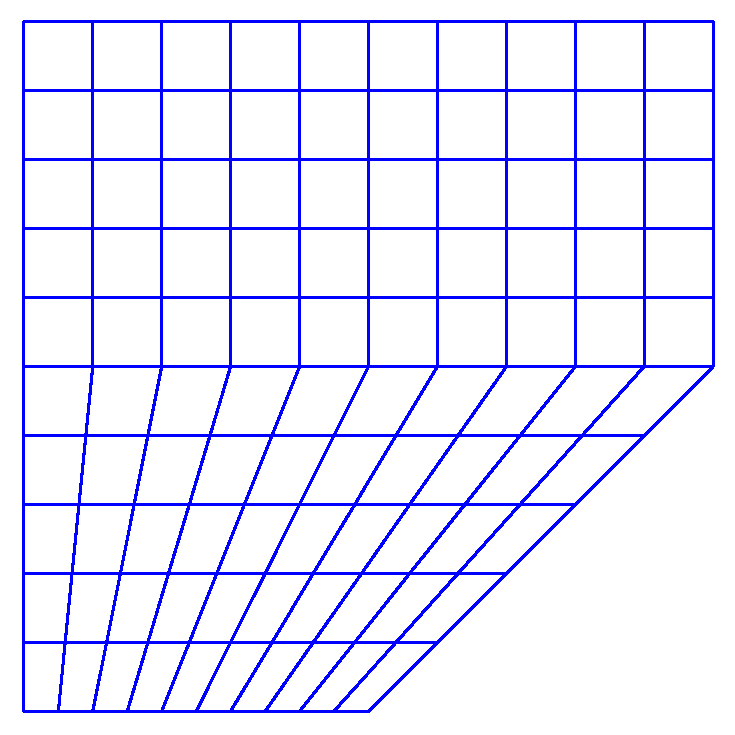
\includegraphics[width=0.45\textwidth]{malla}
\end{center}
\end{document}
